\documentclass[12pt]{article}

\usepackage{times}
\usepackage{graphicx}
\usepackage{appendix}
\usepackage{url}
\usepackage[usenames,dvipsnames]{color} 
\usepackage{float}

\definecolor{mygrey}{gray}{.96} % Light Grey

\setlength{\textwidth}{6.5in}
\setlength{\textheight}{9.0in}
\setlength{\topmargin}{-.5in}
\setlength{\oddsidemargin}{-.0600in}
\setlength{\evensidemargin}{.0625in}

\newcommand{\secref}[1]{Section~\ref{#1}}

\newcommand{\doublespace}{\baselineskip0.34truein}
\newcommand{\singlespace}{\baselineskip0.16truein}
\newcommand{\midspace}{\baselineskip0.24truein}
\newcommand{\midplusspace}{\baselineskip0.26truein}

       
\begin{document}
\begin{titlepage}

\begin{center}


% Upper part of the page
\includegraphics[width=6in]{./Images/logo.png}\\[1cm]    

\textsc{\LARGE Senior Design Project}\\
\textsc{\Large Progress Report 2}\\[0.25cm]
Department of Computer Science and Engineering\\
University of Nebraska-Lincoln\\
CSCE 489\\[0.5cm]

Brett Baumert\\
\textit{bbaumert@gmail.com}\\[0.5cm]

Curtis Johnson \\
\textit{curtisdavidjohnson@gmail.com}\\[0.5cm]
		
Michael Kelly \\
\textit{michael@mikeryankelly.com}\\[0.5cm]

\author{Brett Baumert\\
		Computer Science and Engineering\\
		University of Nebraska-Lincoln\\
		\textit{bbaumert@gmail.com}
	\and
		Curtis Johnson \\
		Computer Science and Engineering\\
		University of Nebraska-Lincoln\\
		\textit{curtisdavidjohnson@gmail.com}
	\and
		Michael Kelly \\
		Computer Science and Engineering\\
		University of Nebraska-Lincoln\\
		\textit{michael@mikeryankelly.com}
}

\vfill

% Bottom of the page
{\large \today}

\end{center}

\end{titlepage}
%\maketitle

\newpage
%\tableofcontents
\newpage
% \doublespace
\section{Introduction}\label{sec:Introduction}

This report discusses the project motivations, functionalities, approaches, quality assurance and risk analysis for our project entitled ODBme.

There were many motivating factors involved in the process in which we finally decided on a specific idea and focus for our senior project.  A common interest in On Board Diagnostics (OBD) was the key factor in the formation of our group. All of us had a general idea of what OBD-II interface was and some of us had even experienced retrieving data from our vehicles via the OBD-II port. We were rather unsure as to what our exact project specifications would be, but from the beginning we knew that we were going to focus our project around the OBD-II technology.

With such a broad project idea, there were a vast number of directions the project could go. OBD-II data is standard on every vehicle post 1996, so there was no concern with the topic focus. The idea of writing applications for mobile devices also entered our minds as a result of the discussion concerning the writing of mobile applications for the bus system. For the simple reason that all three of our group members have Android phones, we quickly became attuned to the idea of writing a mobile application for Android that would somehow connect with the OBD-II port of a vehicle and do many things with the data retrieved.

After some research, we realized that Bluetooth would be the ideal technology to transmit data between the OBD-II device and the Android powered mobile phone. Thus, our project focus was established.

Our project would have both a hardware aspect as well as a software aspect. The Bluetooth transmitter that interfaced with the OBD-II port would be the hardware aspect of our project, and the Android mobile application as well a server side application would make up the software portion of our project.  A more detailed description is given later in this report.  Expanding our project to the scope of using it on other modes of transportation is not our main focus, but it could possibly be done if time allows.

Overall, our motivations came from the desire to incorporate OBD-II data and an Android application together. All of us are very interested in these technologies and feel that a very successful project can come from them.

\section{Projected Functionality}\label{sec:ProjectedFunctionality}
The projected functionalities described in the following paragraphs reference the OBDme architecture as a whole.  This architecture consists of many components, including the OBD-II vehicle connector (hardware), the OBDme Android application, and the OBDme web application.  All components of the OBDme system are explained later in this document.

\begin{figure}[H]
\begin{center}
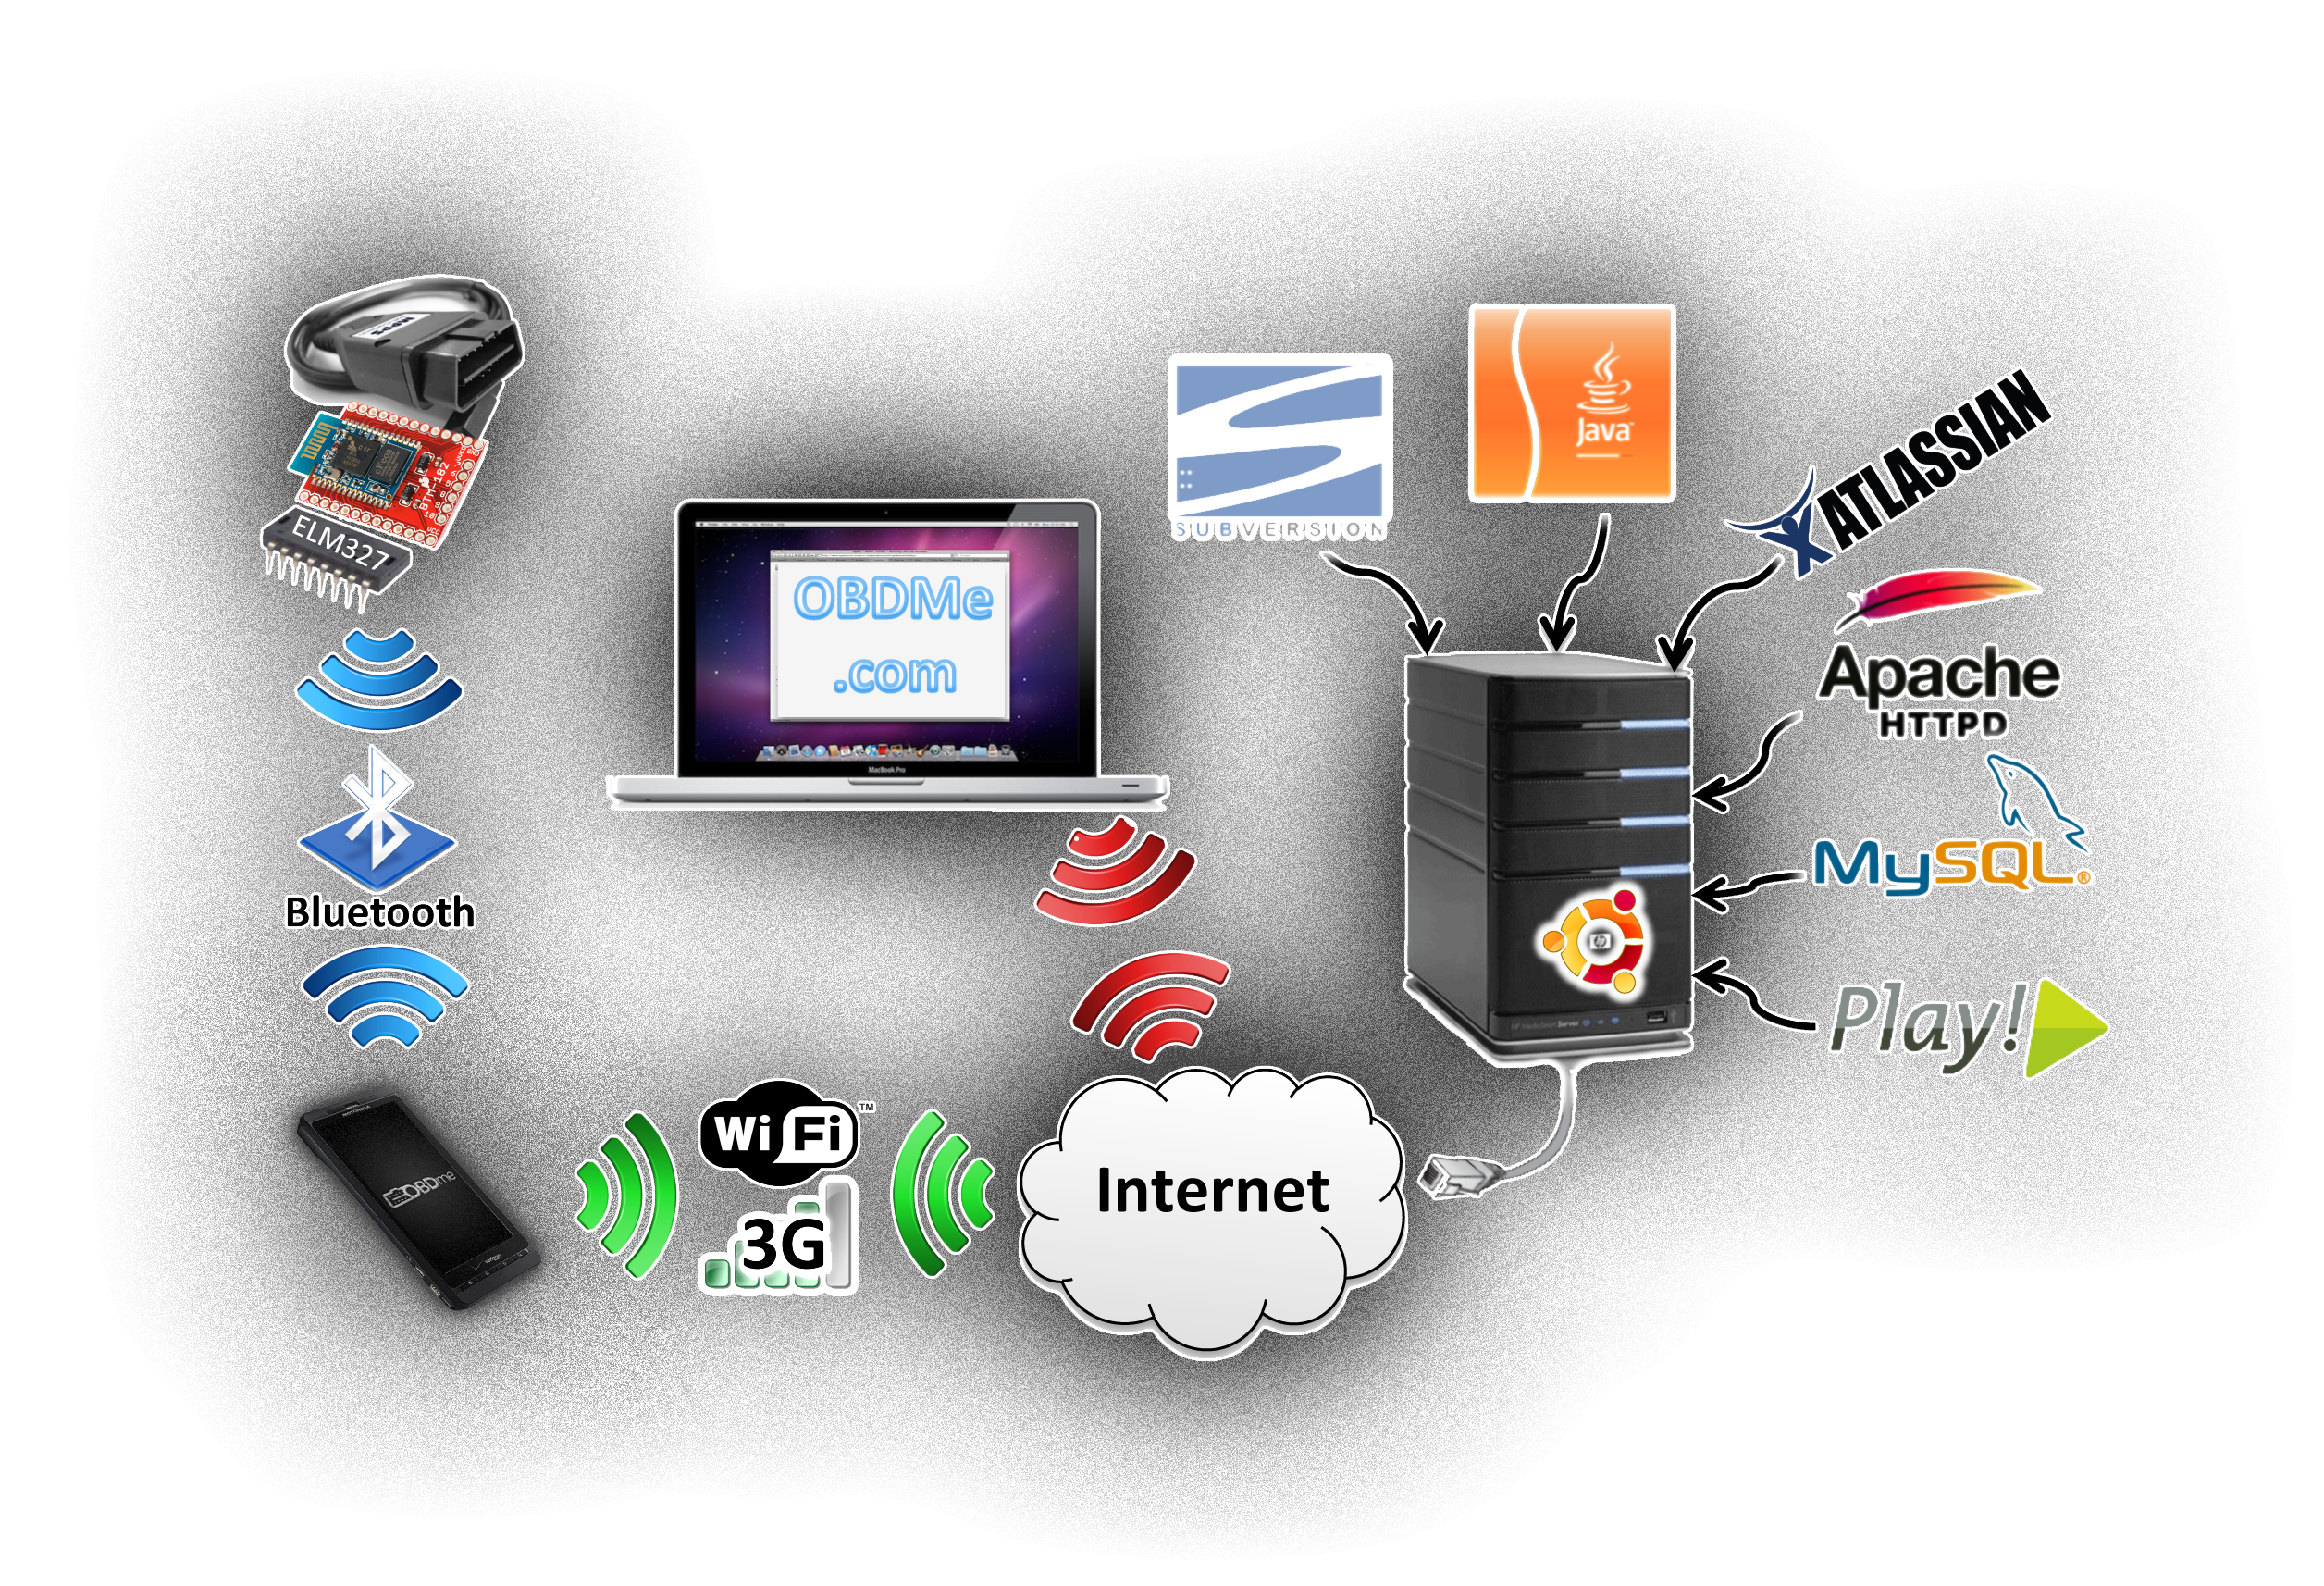
\includegraphics[width=5.5in]{Images/Diagram.png}
\caption{This figure shows the overall architecture of OBDme.}
\label{diagram}
\end{center}
\end{figure}

\subsection{Android Application}\label{subsec:AndroidApplication}
The Android application is both a data collector/logger and a means of displaying data to a user through different modes of operation.  On the initial launch of the Android application, the user will begin an initial setup wizard which will guide the user through the beginning stages of using the OBDme system.  These stages include account creation, Bluetooth capability and configuration, and vehicle registration.  This process will ensure that the user can easily configure the application, even while having little knowledge of Android, Bluetooth, or the OBD-II protocol.  While the setup wizard is very helpful to the end-user, it is also helpful to the OBDme application.  The setup wizard, unknowing to the user, will take steps to verify that the hardware the user has chosen to use is entirely compatible with the OBDme application.  Images of the setup wizard can seen below.

\begin{figure}[H]
\begin{center}
\includegraphics[height=3.5in]{Images/setup_wizard.png}
\includegraphics[height=3.5in]{Images/setup_wizard_vin.png}
\caption{The figure on the left shows the setup wizard after connecting to the OBD hardware via Bluetooth.  The figure on the right shows the setup wizard after initial communication with the vehicle's on-board computer}
\label{setup_wizard}
\end{center}
\end{figure}

The Android application will offer multiple user modes.  The first mode of operation is considered the basic user mode.  In this mode of operation, real-time data is displayed to the user in a simple but effective manner.  In the portrait orientation, two values are displayed at any given time, whereas only one value is displayed at a time in landscape orientation.  This minimalistic user interface was designed with the safety of the user in mind.  Values are displayed in large, easy to read fonts to keep the attention away from the application and the focus on operating the motor vehicle.  Images of the basic user mode can be seen below.

\newpage

\begin{figure}[H]
\begin{center}
\includegraphics[height=3.5in]{Images/basic_mode_portrait.png}
\includegraphics[width=3.5in]{Images/basic_mode_landscape.png}
\caption{This figure shows real-time data collection in a portrait orientation and landscape orientation.}
\label{basic_mode}
\end{center}
\end{figure}

The second user mode is the advanced user mode.  In this mode, users will be able to view a list of real-time data as opposed to just one or two pieces of data.  This list of data will be very useful to those who wish to analyze multiple instantaneous values.  This mode is a combination of two earlier proposed "enthusiast" and "mechanic" modes.  Individual data values may be selected from the list to view more information about a specific value, or to transition to a real-time plot or graph of the recorded values.

While in the application, the user will have a great amount of control, choosing which user "mode" they would prefer to use.  In each of these modes of operation, the user can simply alter their application preferences to set a various number of options.  Within these preferences, one of the most important items a user may control is the types of vehicle data that are displayed in the application.  This will give users the ability to disregard data they are not interested in, and only show the data that is important.  Other application preferences include items such as choosing when to upload vehicle data based on the user's connection type (3G, Wifi, etc).

Along with these use cases of displaying real-time data, another set of use cases involve the retrieval of certain problems that may arise with a vehicle.  These problems often cause a "Service Engine Soon" or "Check Engine" light to appear inside of the vehicle.  The OBDme application would allow the user to view a simple description of the problem at hand, and may possibly suggest a solution for the problem to the user.

\subsection{Web Application}\label{subsec:Web Application}
Another important application component, of the OBDme system, is the web application. The web application will be the primary data consumer of all collected data from the OBDme Android application. The web application will focus on bringing the most important and valuable pieces of collected data together in an easy to understand format for the user. For instance, the user may simply want to view the average RPM (revolutions per minute) reading from the data available to the OBDme system. Many graphs like this will be obtainable to the user through the web application.

The web application will function like many other web applications.  The user will first have to log in using a username and password, or they will have to create a username and password if one is not already created.  Once logged in, the user will be able to interact with the OBDme web application in numerous ways.  Account settings and information can be added or changed via the “profile” page.  The main function of the web application is to allow the user to view the statistics about their vehicle(s) which they have logged using the OBDme Android application.  A “statistics” page can be accessed to do this, and there will be a filtering system in place to allow the user to easily view only the information they desire.  Some screenshots of the web application can be seen below.

\begin{figure}[H]
\begin{center}
\includegraphics[width=5.5in]{Images/login_page.png} 
\caption{This image shows the login page at www.obdme.com.}
\label{hardware}
\end{center}
\end{figure}

\begin{figure}[H]
\begin{center}
\includegraphics[width=5.5in]{Images/control_panel.png} 
\caption{This image shows the control panel used to navigate the website.  This control panel can be collapsed to allow full view of the page.}
\label{hardware}
\end{center}
\end{figure}

Another key function of the web application involves a concept of "trips". The user will first have to specify that they want to record a trip via the Android application.  The Android application will then associate all data collected with that trip.  The user will then have to signify the end of the trip via the Android application, and in the same manner as they began the trip. The data collected between the time the user starts the trip and when the user stops the trip will be associated with the trip when the data is viewed on the web application.

The data trends and graphs displayed on the web application will be the key factor that separates the web application from the Android application.

\section{Proposed Approaches}\label{sec:ProposedApproaches}

\subsection{Hardware Interface}\label{subsec:HardwareInterface}
The core goal of our project is to interface with any standard OBD-II port that has been equipped in vehicles since 1996. Initially, we had a couple approaches to this problem but eventually converged on one single approach.

Serial communication with the OBD-II port seemed to be the best approach to take.  A chip currently on the market called the ELM327, that is manufactured by ELM Electronics made this a possibility.  The ELM327 chip connects to the ODB-II port and enables RS-232 communication with the OBD-II port. With some additional circuitry, the ELM327 is the core logic element of our hardware implementation. It provides an easy and abstracted means of communicating with all OBD-II protocol standards.

For end user simplicity, we chose to implement wireless connection between the end device and the ELM327. For short range and reliable communication, Bluetooth was chosen as the wireless protocol of choice. A Bluetooth module was interfaced with the RS-232 elements of the ELM327 chip, and acts as a transparent carrier between the ELM327 and any connected device.

Additional circuitry was added to provide the Bluetooth and ELM327 IC's with adequate operating power. Since these components require different operating voltage levels, regulators were used to decrease the standard 12V vehicle power supply to the adequate voltages the circuit components require.

A picture of the Bluetooth enabled OBD-II transceiver, which we constructed, can be seen below.

\begin{figure}[H]
\begin{center}
\includegraphics[width=5.5in]{Images/hardware_with_labels.png} 
\caption{This image shows the hardware implementation of our project.}
\label{hardware}
\end{center}
\end{figure}

\subsection{Android Application}\label{subsec:AndroidApplication}

The next core design element of our project is an Android application.  The Android application will have several main functions. First, the application will act as a data display for the OBDme hardware.  For the basic subset of users the application will display simple statistics such as acceleration, deceleration, fuel efficiency, and vehicle health.  For the more advanced subset of users the application will display additional information such as average and instantaneous diagnostic values from the vehicle.  For this data to be displayed, it must first be collected.  Thus, a good majority of the underlying pieces of the Android application are dedicated to communicating with the hardware interface mentioned above.  The application obtains the vehicle data from the hardware interface, makes the data available to the user interface, and finally stores the data to a temporary database located on the phone.

The phone will act as a data transceiver.  Specifically, the application will determine what data is available from the vehicle and then transmit that available data to some remote service.  This operation happens as a background process.  A collector will continuously pull diagnostic information from the vehicle (as mentioned above) and store it locally until (signal strength permitting) it can be uploaded to a remote web service.  Once this data is uploaded to the remote web service, it is flushed from the phone.

Communication with the remote OBDme data service will send and consume messages in the JSON (Javascript Object Notation) format.  This format is an industry standard in HTTP communication.  Initially Google Gson was used for JSON processing.  With some research and testing, a much quicker processor was discovered.  This processor is called Jackson.  Using Jackson instead of Gson, helped the speed and resource usage of our application immensely.  The speed of JSON processing is very important since one of the main functions of the Android application is sending data to the web
server, or remote OBDme data service.  A speed comparison chart can be seen below.

\begin{figure}[H]
\begin{center}
\includegraphics[width=5.5in]{Images/json_compare.png} 
\caption{This image shows a speed comparison between Google GSON and Jackson JSON parsers.  Both serial and streaming cases were tested.}
\label{hardware}
\end{center}
\end{figure}

\subsection{Data Storage}\label{subsec:DataStorage}
Once we have successfully interfaced with the OBD-II port on the vehicle, we will be able to obtain large amounts diagnostic data. This data will be valuable whether the end user is interested in average/instantaneous statistics, or other data relevant to troubleshoot engine problems. After all of this data is collected from the vehicle, it will be stored and possibly used for analysis a later time. 

For a small implementation discussed in this project, a large clustered storage solution will not be required. Regardless, we will need a dependable solution for storing this data as the data may be vital towards future statistical analysis. The most ideal solution will be to store diagnostic data using an off the shelf (OTS) commercial database application.

Any outside applications will not be able to interface with the database directly, so a gateway will need to reside in front of our database to accept and retrieve queries for clients. This gateway would in essence be a web service that varies depending upon our application needs. Using these services, we can also handle authorization and other security-related issues. These security related issues will be crucial in safe guarding user information and data.

Data will be stored locally on the phone as it is collected. Android provides an SQLite database that will work for this purpose.  This storage is only temporary.  The data is placed in a queue until it can be sent to the web server.  Once the data gets sent to the web server it is deleted from the temporary storage on the phone.  The user has the ability to set a preference, which controls how the data is sent to the web server.  The data can be sent either by a wifi connection, or a phone data network connection (3G or 4G) when either is available.  Most Android phones have plenty of storage, so if the data is not immediately uploaded to the web server, it will just remain in the phone’s storage.

\subsection{User Interaction}\label{subsec:UserInteraction}
As a compliment to the previously discussed Android application, we would like to be able to present any data retrieved from a specific vehicle to a user through a web interface.  By providing data in the fashion, a user would have a intuitive way to view statistics about their vehicle and driving habits using a more fully featured device with a larger display.  Potentially, this interface might be used the same by mechanics to diagnose vehicular problems. 	 

To present these statistics to the user, we will use a variety of web standards to provide compatibility for many devices ranging from desktop computers to mobile devices.  For this reason, we will develop a web application using HTML5 to allow the user to interact with their statistics.

\subsection{Server Architecture}\label{subsec:ServerArchitecture}

For the back-end aspect of the entire system, we will require many dependable yet cost-effective solutions to keep the system responsive as well as easy to use.  It is easy to see that the database could be possibly the most vital part of the back-end.  Because of this, we have chosen to use an industry standard database system.  MySQL fulfils many of our requirements, since it is cost effective (free), and also very dependable.

A sturdy web service structure and web application is also as important as the database for the full operation of this system.  To implement these aspects of the project, we have chosen to use Java for our web framework, since it is also cost effective (free), dependable, and very familiar to the developers.  More specifically, the Play! framework for Java web development will be used.  Play!, an MVC (model-view-controller) framework, will easily allow for development of the web application and the data services side by side, in the same application.

Earlier it was mentioned that communication messages between the data service and the \\ OBDme phone application will mainly utilize the JSON format.  This format was chosen for its condensed size, out-of-the-box operability with Java, and for its industry-wide reputation.  By using a format as well known as JSON, the data services may be developed with expandability in mind, as many frameworks can utilize JSON.  In the future, other companies and/or applications may be able to consume the data services, allowing OBDme to grow in ways never imagined.

\section{Quality Assurance}\label{sec:QualityAssurance}
Testing will be a very important part of the design and implementation of our project.  Because of the many different aspects, and the complexity of our project, testing will be performed quite often.  Unit testing, integration testing, and system level testing will be present at each stage of design and implementation.

Unit testing will be the most important part of our development strategy.  Identifying problems early is vital to the success of the end product.  For this reason, we plan unit test every aspect of OBDme.  The OBD-II hardware interface will be tested thoroughly, mainly by way of test programs run from a computer.  These tests could test routine commands, as well as edge cases (the program may request a diagnostic value the vehicle does not support, or can not return).

The Android application will also be unit-tested thoroughly.  However, the application will be highly dependent upon the hardware interface.  Much of the unit-testing of the Android application will need to handle cases such as Bluetooth connection problems, Internet connection problems, etc.

Finally, each individual aspect of the server side implementation (database, web application, learning algorithms) will also be unit tested.  While the database and web application will have rather simple unit tests, the learning algorithms will require very intensive unit tests, which will be performed as time permits.

Integration testing will be performed during development as well.  These will including many aspects of the OBDme system.  The Android application communicating with the hardware interface will be tested thoroughly.  The web services / API will be tested communicating with the database.  The Android application will also be tested communicating with the APIs.  The web application will need to be tested communicating with the database as well.

Finally, system level testing will take place towards the end of OBDme development.  System level testing will examine many use cases.  For example, this testing may involve retrieving information from the vehicle via the Android application, logging the data to the sever, and finally viewing the data via the web application.  There will be numerous system level tests performed, but will not be fully realized until development has progressed and integration testing is well under-way.

\section{Risk Analysis}\label{sec:RiskAnalysis}

There are many potential risks that are presented with a project of this size and scope.   The risks discussed below only represent the immediately identifiable potential risks.  What is also of concern is the risks that are not identified and discussed in this report.  Regardless of all potential risks, we are confident that we will be able to overcome them and complete the project on time and in full.

With a team of three senior computer engineering undergraduate students, schedules are very tight.  Each team member has full course schedule with their own respective set of homework assignments, projects, and other obligations.  Each team member is also employed in a part time job, further decreasing our available time.  While our senior design project holds a very high importance, it can not dominate our academic or personal schedules.  Navigating around these issues will be difficult without excellent time management.  We have created a shared team calendar to facilitate collaboration, scheduling work, and to find common free time.

Our group has no way to anticipate the outcome or limitations of both hardware and software components used in the project.  However, from our combined experience in both the academic and corporate environments, we have learned to expect these potential problems in advance.  We are confident that what we are trying to accomplish using hardware is feasible given that commercial products with the same capabilities are already available.  We also free that utilizing widely used open source software in our project design makes a great deal of technical resources available to us.

Despite the potential risks when considering the hardware and software in our project, there is also a significant amount of potential physical risks involved as well.  The sensor data we collect and our mobile application interface is dependent on real sensor values, testing these things in a moving automobile introduces potential safety risks, especially when the tester and driver are the same person.  We need to place a significant importance on driving safety because, not only are we putting ourselves at risk, but other individuals as well.  Testing our device and software with OBD-II error codes means, we will be causing intentional mechanical problems with a car.  We will need to ensure that these intentional problems will not permanently damage the engine and that it will not place us or others at risk when driving the vehicle. 

Earlier in the development of the OBDme system, as a result of the amount of hardware and software used in the project, it was noted that unfamiliarity with the several platforms involved could have resulted in lost development time required for training and familiarization of all hardware and software platforms.  The solution was for members to become experts on their assigned technologies, compared to all members having a vague knowledge of all technologies.  This has in fact decreased the learning curve for the team, and increased the development rate for the project as a whole.

Considering all of the potential risks above and the unforeseeable risks not mentioned, we are confident that acknowledging them in advanced will allow us to compensate for them in the future.  Realizing these risks now will also allow us to correctly manage our time in the future so that we meet all of our projected goals.

\section{Project Plan}\label{sec:ProjectPlan}

During the project development phase, several commercially available management tools will be used.  The first, is an issue management tool called JIRA.  JIRA will allow us to set deadlines, open and close project issues, assign tasks as well as many other management related issues.  Each task in JIRA can be assigned to a specific person.  This will keep people in charge of and responsible for certain aspects of the project.  All team members can use this tool to track the other team member progress as well.

Fisheye and Crucible are tools similar to JIRA that will allow group members to view each others software contributions.  These tools also allow for simple and effective code reviews.  This will be a great opportunity for the group to audit one another's code contributions in a fast and less humiliating way than traditional code reviews.  An example figure of JIRA is shown below.

\begin{figure}[H]
\begin{center}
\includegraphics[width=6.5in]{Images/jira.png} 
\caption{This figure shows an example of our JIRA installation. Projects inside the JIRA tool are show to the right and an activity stream is shown on the left.}
\label{jira}
\end{center}
\end{figure}

Instead of providing a weekly schedule, we will provide a slightly broader plan for our project objectives and stages.  During each weekly meeting the previous week's progress will be evaluated and goals for the following week can be adjusted based on the previous weeks performance.  JIRA, Crucible, and Fisheye will allow us to adapt project deadlines around our real world schedules and other unforeseen complications.

\subsection{Monthly Target Dates}\label{subsec:MonthlyTargetDates}

%\begin{description}
%	\item[March 31, 2011] Android application nearing completion, and E-Week Preparation.
%	\item[April 30, 2011] Web application complete, and finalize testing of applications (Android and Web).
%\end{description}

%\bibliographystyle{plain}
%\bibliography{Proposal.bib}
%\newpage
%\section{Appendix}\label{sec:Appendix}
%\newpage
%\appendix


\begin{figure}[H]
\begin{center}
\includegraphics[width=5.5in]{Images/schedule_march_april.png} 
\caption{This image shows our current overall schedule for the report.}
\label{schedule}
\end{center}
\end{figure}

\end{document}